\documentclass{bioinfo}
\copyrightyear{2005}
\pubyear{0000}

\begin{document}
\firstpage{1}

\title[short Title]{R/DWD: Distance Weighted Discrimination and Second
  Order Cone Programming} \author[Sample \textit{et~al}]{Hanwen
  Huang\,$^{1,2,3}$\footnote{to whom correspondence should be
    addressed}, Xiaosun Lu\,$^{1,2}$, Yufeng Liu\,$^{1}$, Perry
  Haaland\,$^{2}$, J. S. Marron\,$^1$ \address{$^{1}$Department of
    Statistics and Operations Research, University of North Carolina
    at Chapel Hill, Chapel Hill, NC 27599 USA.\\ $^{2}$BD
    Technologies, 21 Davis Drive, RTP, NC 27709 USA.\\$^{3}$University
    of Texas Health Science Center at Houston, Houston, TX 77030
    USA.}}

\history{Received on XXXXX; revised on XXXXX; accepted on XXXXX}

\editor{Associate Editor: XXXXXXX}

\maketitle

\begin{abstract}

\section{Summary:}
R/DWD is an extensible package for classification and optimization. It
provides a new classification tool using a recently developed Distance
Weighted Discrimination (DWD) method which is related to, but has been
shown to be superior to, Support Vector Machine (SVM) in some high
dimensional situations.  The key step in the implementation of DWD is
to solve a Second Order Cone Programming (SOCP) problem. R/DWD also
provides an efficient SOCP solver based on the interior point method
originally developed by Toh {\em et al.}, 1999 for solving
semidefinite-quadratic-linear programming. In addition, an efficient
Quadratic Programming solver based on the SOCP is also included in
this package. We believe that this package will be very useful for
many aspects of bioinformatics research.

\section{Availability:} The package is freely available from cran.r-project.org.

\section{Contact:} \href{hanwen.huang@uth.tmc.edu}{hanwen.huang@uth.tmc.edu} or
\href{Perry\_Haaland@bd.com}{Perry\_Haaland@bd.com}
\end{abstract}

\section{Introduction}

The Support Vector Machine (SVM) is a well known machine learning
technique and has achieved great success in bioinformatics
applications (see Byvatov {\em et al.}, 2003 for a review). However,
as shown in Marron {\em et al.}, 2007, SVM suffers from the data
piling problem in High Dimensional Low Sample Size (HDLSS) situations.
Distance Weighted Discrimination (DWD) is a recently developed
classification method which was originally motivated for solving the
HDLSS problems (Marron {\em et al.}, 2007), but can be applied to many
other examples as well. One of the big advantages of DWD over SVM is
that it can overcome the data piling problem in high dimensional
situations as illustrated in Figure \ref{dwdsvm}. The original DWD
paper (Marron {\em et al.}, 2007) only described the implementation of
the binary classification method. The multiclass version of DWD has
also been developed in Huang {\em et al.}, 2011. It is suggested that
all users refer to these publications in order to understand the DWD
terminology and principles in greater detail.

\begin{figure}[ht]
\begin{center}
\includegraphics[keepaspectratio=true, width=0.5\textwidth]{mdp.ps}
\caption{Superior Performance of DWD over SVM in HDLSS settings. The
  toy example has dimension $d=50$, with $n_+=20$ data vectors from
  Class +1 (red plus signs), and $n_-=20$ data vectors from Class -1
  (blue circles). The data were drawn from 2 distributions that are
  nearly standard normal, except that the mean in the first dimension
  is shifted to +2.2 (-2.2) for Class +1 (-1). Four important
  one-dimensional projections are shown here with the horizontal
  coordinate representing the projection, and with a random vertical
  coordinate used for visual separation of the points. The top left,
  top right, bottom left and bottom right are the projections onto the
  true optimal, Maximum Data Piling (MDP, Ahn {\em et al.}, 2010), SVM
  and DWD directions respectively. The DWD direction is closer to the
  optimal direction than the SVM direction as indicated by both the
  kernel density estimation (solid curve) and the calculated angle to
  the optimal direction. The Maximum Data Piling direction in HDLSS is
  illustrated by the top right plot.}
\end{center}
\label{dwdsvm}
\end{figure}

DWD has been widely used in many bioinformatics areas including
adjusting batch effects in microarray expression data (Benito {\em et
  al.}, 2004) and discovering cancer subtypes (Hu {\em et al.},
2006). However, the existing DWD package was written in Matlab which
is not a free software package. To make it more convenient for
bioinformatics people to use, we have developed an R version of DWD
here. R/DWD is based on the existing Matlab version
(http://www.unc.edu/$\sim$marron/marron\_software.html), but includes
some additional features such as multiclass version. For the
convenience of the users who are familiar with using SVM in R, the
main classification functions and arguments in \texttt{R/DWD} are
formatted in a similar way to the ones used by the corresponding SVM
functions in the \texttt{kernlab} package. To help the users in using
this software, some examples to illustrate the coding are provided.

\section{Optimization Algorithm}
The implementation of DWD is more challenging than the implementation
of SVM because it requires solving an optimization problem called
Second Order Cone Programming (SOCP).  The DWD Matlab version employed
a very efficient SOCP solver from the \texttt{SDPT3}
(semidefinite-quadratic-linear programming) package developed by Toh
{\em et al.}, 1999. The \texttt{SDPT3} implemented an infeasible
path-following algorithm for solving conic optimization problems
involving semidefinite, second-order and linear cone constraints.

Central to R/DWD is the SOCP solver which was implemented using
exactly the same algorithm as the one used by the corresponding Matlab
version. The optimization problem that underlies SVM is called
Quadratic Programming (QP). An efficient R/QP solver based on the SOCP
is also included in this package which provides a useful tool for
those users who want to make their own modifications of the SVM
method.

\section{Features}

\subsection{Classification}
Both SVM and DWD are margin-based classification methods in the sense
that they build the classifier through finding a decision boundary to
separate the classes (Liu, {\em et al}, 2011). DWD uses a different
criterion from SVM. It seeks to achieve the goal by maximizing the
average distance rather than the minimum distance among the
classes. Similar to the \texttt{ksvm} function from \texttt{kernlab},
which has been widely used in SVM analysis, we developed a function
called \texttt{kdwd} in this package for doing DWD analysis.

To solve multiclass classification problem, two different methods are
used. The first one is to use the ``one-versus-one" approach, in which
classifiers are trained on each pair of classes and the class label is
predicted by a voting scheme. The second one is to build a single
classifier including all classes simultaneously and solve a big
optimization problem.

Every DWD analysis requires two elements from a dataset: (1) a matrix
of predictors, which should be in the form of an $n \times d$ matrix,
where $n$ represents the sample size and $d$ represents the
dimension. (2) a response vector of length $n$ with each element
corresponding to one sample. The appropriate scaling steps can be
taken by using the \texttt{scaled} option. It should be noted that in
the current version of \texttt{DWD}, missing values are not allowed,
and must be imputed prior to analysis.

The basic output from \texttt{kdwd} is an object of class {\em
  kdwd}. Showing objects of class {\em kdwd} will print details on the
results for all classifiers included in the model. For each
classifier, the optimal solution of the parameters are displayed along
with the final primal and dual objective values.  The cross validation
error rate can also be returned with the argument \texttt{cross = k},
where \texttt{k} is the number of folds used in the cross-validation.

\subsection{Optimization}
The application of SOCP is not limited to DWD, it can be used to solve
many other problems as well. The package \texttt{R/DWD} provides a
stand-alone SOCP solver called \texttt{sqlp}. The algorithm
implemented in \texttt{sqlp} is an infeasible primal-dual
path-following algorithm, described in detail in Toh {\em et al.},
1999. The basic idea is that, at each iteration, we first compute a
predictor search direction aimed at decreasing the gap between the
primal and dual objective values. After that, the algorithm generates
a corrector step with the goal of keeping the iterations close to the
central path. The most crucial part is to solve a linear system which
is especially challenging in situations when a big sparse matrix is
included. To increase the speed and efficiency, the sparse matrix
package \texttt{Matrix} is incorporated to deal with high dimensional
large datasets.

QP is a special case of SOCP. SVM is only one of the important
applications of QP, but QP can be applied to many other areas as
well. The QP solver in this package is formatted in a similar way but
has been shown to be more numerically stable than the existing QP
solver \texttt{solve.QP} in \texttt{quadprob} package.

\section{Discussion}
The main purpose of R/DWD is to do classification and optimization,
both of which are very important in bioinformatics fields. In
classification, the DWD method is implemented. In optimization, the
efficient SOCP and QP solvers are provided which can be integrated
into a variety of applications. R/DWD is under continual
development. Only the linear discrimination method is considered in
the current version. Future plans include incorporating some kernel
tricks into the DWD method such that it can be used to solve more
general nonlinear problems. In addition to prediction of class labels,
we are also investigating ways to predict the probability of a data
point belonging to a certain class based on the given
measurements. Moreover, we also intend to develop some imputation
methods to handle missing values in the input file.

\begin{thebibliography}{}

\bibitem[Ahn, 2010]{ahn2011}Ahn, J. and Marron, J. S. (2010),
  \textit{The Maximal Data Piling Direction for Discrimination},
  Biometrika, 97(1):254-259
\bibitem[Byvatov, 2003]{byvatov2003}Byvatov E, Schneider G. (2003),
  \textit{Support vector machine applications in bioinformatics}, Appl
  Bioinformatics. 2003;2(2):67-77.
\bibitem[Benito, 2006]{benito2006}Monica Benito, Joel Parker, Quan Du,
  Junyuan Wu, Dong Xiang, Charles M. Perou, and J. S. Marron (2004),
  \textit{Adjustment of systematic microarray data biases},
  Bioinformatics (2004) 20 (1): 105-114.
\bibitem[Hu, 2006]{hu2006}Hu Z, Fan C, Oh DS, Marron JS, He X, Qaqish
  BF, Livasy C, Carey LA, Reynolds E, Dressler L, Nobel A, Parker J,
  Ewend MG, Sawyer LR, Wu J, Liu Y, Nanda R, Tretiakova M, Ruiz Orrico
  A, Dreher D, Palazzo JP, Perreard L, Nelson E, Mone M, Hansen H,
  Mullins M, Quackenbush JF, Ellis MJ, Olopade OI, Bernard PS, Perou
  CM. \textit{The molecular portraits of breast tumors are conserved
    across microarray platforms}. BMC Genomics. 2006 Apr 27;7:96.
\bibitem[Huang, 2011]{huang2011}H. Huang, Y. Liu, Y. Du, C.M. Perou,
  D.N.  Hayes, M.J. Todd, and J.S. Marron, (2011), \textit{Multiclass
    distance weighted discrimination with applications to batch
    adjustment}, submitted.
\bibitem[Karatzoglou, 2011]{Karatzoglou}Alexandros Karatzoglou, Alex Smola,
  Kurt Hornik, \textit{Kernel-based Machine Learning Lab}, CRAN -
  Package kernlab.
\bibitem[Liu, 2011]{liu2011}Liu, Y., Zhang, H. H., and Wu, Y. (2011).
  \textit{Soft or hard classification? Large margin unified
    machines}. Journal of the American Statistical Association, 106,
  166-177.
\bibitem[Marron, 2007]{marron2007} Marron, J. S., Todd, M. J. and
  Ahn,J., (2007), \textit{Distance-Weighted Discrimination}. Journal
  of the American Statistical Association, Vol. 102, No. 480,
  pp. 1267-1271.
\bibitem[Toh, 1999]{toh1999}K.C. Toh, M.J. Todd, and R.H. Tutuncu,
  \textit{SDPT3 --- a Matlab software package for semidefinite
    programming}, Optimization Methods and Software, 11 (1999),
  pp. 545--581.
\bibitem[Turlach, 2011]{turlach}Berwin A. Turlach, \textit{quadprog:
  Functions to solve Quadratic Programming Problems}, CRAN - Package
  quadprog

\end{thebibliography}
\end{document}
